% flashcards-title: Measurement interval and two model predictions
% flashcards-desc: A shaded reported interval extends from 9.8 to 10.2 centimetres. Triangular prediction A is at 10.1 centimetres inside the interval; square prediction B is at 10.5 centimetres outside it.
\documentclass[border=6pt]{standalone}
\def\pgfsysdriver{pgfsys-dvisvgm.def}
\usepackage{tikz}
\usetikzlibrary{arrows.meta,positioning,shapes.geometric}
\definecolor{mechInk}{HTML}{172033}
\definecolor{mechBlue}{HTML}{155EEF}
\definecolor{mechOrange}{HTML}{B54708}
\definecolor{mechPale}{HTML}{E8F0FF}
\definecolor{mechGray}{HTML}{667085}
\definecolor{mechLight}{HTML}{D0D5DD}
\tikzset{
  every picture/.style={font=\sffamily\large, text=mechInk},
  mech box/.style={draw=mechInk, line width=1.2pt, rounded corners=4pt,
    fill=white, align=center, minimum height=14mm, inner xsep=5mm},
  mech primary/.style={draw=mechBlue, line width=2.2pt},
  mech secondary/.style={draw=mechOrange, line width=2.2pt, dashed},
  mech guide/.style={draw=mechGray, line width=0.9pt, dashed},
  mech arrow/.style={-{Stealth[length=3.2mm,width=2.4mm]},
    draw=mechInk, line width=1.4pt, line cap=butt},
  mech axis/.style={draw=mechInk, line width=1.2pt},
  mech tick/.style={draw=mechInk, line width=1pt}
}

\begin{document}
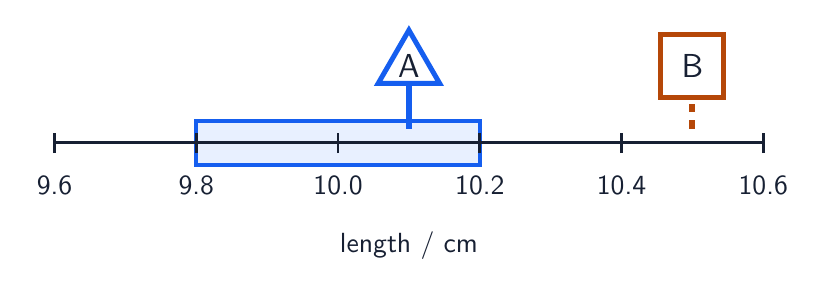
\begin{tikzpicture}[x=9cm,y=1cm]
  \fill[mechPale] (0.2,-0.28) rectangle (0.6,0.28);
  \draw[mechBlue, line width=1.5pt] (0.2,-0.28) rectangle (0.6,0.28);
  \draw[mech axis] (0,0) -- (1,0);
  \foreach \x/\lab in {0/9.6,0.2/9.8,0.4/10.0,0.6/10.2,0.8/10.4,1/10.6}{
    \draw[mech tick] (\x,-0.13) -- (\x,0.13);
    \node[below=3mm, font=\sffamily\normalsize] at (\x,0) {\lab};
  }
  \node[below=10mm, font=\sffamily\normalsize] at (0.5,0) {length / cm};
  \draw[mech primary] (0.5,0.18) -- (0.5,0.72);
  \node[draw=mechBlue, fill=white, regular polygon, regular polygon sides=3,
    line width=1.8pt, minimum size=9mm, inner sep=0pt] at (0.5,0.98) {A};
  \draw[mech secondary] (0.9,0.18) -- (0.9,0.72);
  \node[draw=mechOrange, fill=white, rectangle, line width=1.8pt,
    minimum size=8mm, inner sep=0pt] at (0.9,0.98) {B};
\end{tikzpicture}
\end{document}
